\ifdefined\ThermalOneD
\documentclass[12pt]{report}
\usepackage{graphicx}
\usepackage{float}
\usepackage[a4paper, margin=1in]{geometry}
\usepackage[utf8]{inputenc}
\usepackage{textcomp}
\usepackage{amsmath}
\usepackage{booktabs}
\usepackage{tikz}
\usepackage{enumitem}
\usetikzlibrary{decorations.pathmorphing,patterns}
\usepackage[hidelinks]{hyperref} % <- hypertext
\usepackage{caption}

% <- Define folder macros for modularity
\newcommand{\RADCONVDIR}{radiation_convection}  % <-Radiative + convection case
\newcommand{\HEATCONDDIR}{heat_conduction}      % Heat conduction 
\newcommand{\HKCDIR}{heat_conduction_kc}        % Heat conduction with K(T) and C(T)
\newcommand{\CONVDIR}{convective_cooling}       % Convective cooling
\newcommand{\STEELDIR}{insulated_steel_plate}   % insulated steel plate
\newcommand{\RADLOSSLDIR}{radiation_loss}       % Radiative loss
\newcommand{\FIXEDDIR}{fixed_temp_sides}        % fixed boundary temperatures
\newcommand{\SURFRADDIR}{radiation_1d}          % Surface radiation
\newcommand{\DEPTHDIR}{radiation_depth}         % Depth radiation
\newcommand{\DEPTHCONVDIR}{rad_conv_depth}      % Depth radiation

\begin{document}
\fi


\graphicspath{
  {\HEATCONDDIR/}
  {\HKCDIR/}
  {\CONVDIR/}
  {\STEELDIR/}
  {\RADCONVDIR/}
  {\RADLOSSLDIR/}
  {\FIXEDDIR/}
  {\SURFRADDIR/}
  {\DEPTHDIR/}
  {\DEPTHCONVDIR/}
}



\chapter{ Thermal 1D}

\newpage
\ifdefined\standalone
\documentclass[12pt]{article}
\usepackage{graphicx}
\usepackage{float}    % <-- For [H] figure placement
\usepackage[a4paper, margin=1in]{geometry} % <-- For better margins
\usepackage[utf8]{inputenc}
\usepackage{textcomp}  % <-- for \textdegree
\usepackage{amsmath}
\usepackage[hidelinks]{hyperref} % <- hypertext
\begin{document}
\fi

\section{Heat Conduction} 
Four distinct cases of one-dimensional transient heat conduction through a $L=$0.1 m thick plate are analyzed. In each case, the plate is initially at a uniform temperature of $T_{ini}=$20\textdegree{}C and is exposed on one side to ambient air at $T_\infty=$120\textdegree{}C with convection, while the other side is perfectly insulated. The key parameters for each case are summarized in the table \ref{tab:cases_properties}. The evolution of the temperature profiles can be seen in fig. \ref{fig:HC_ABCD}.


The Analytical temperature field in the plate is given by Incropera et al \cite{incropera_fundamentals_2007}:
\begin{equation}
T(z,t) = T_\infty + (T_{ini} - T_\infty)\sum_{n=1}^{\infty} C_n \cos\!\left(\beta_n \frac{z}{L}\right)
\exp\!\left(-\beta_n^2 \frac{\alpha t}{L^2}\right)
\label{Eq:Thermal_thranscendantale}
\end{equation}
where $\alpha = k/(\rho c)$ is the thermal diffusivity, $C_n = \dfrac{4\sin(\beta_n)}{2\beta_n + \sin(2\beta_n)}$ a constant, and the eigenvalues $\beta_n$ satisfy $\beta_n \tan(\beta_n) = Bi$, where $Bi$ is the Biot number.

\vspace{-0.5cm}

\begin{table}[H]
\centering
\caption{Properties for Each Heat Conduction Case}
\label{tab:cases_properties}
\begin{tabular}{|l|c|c|c|c|}
\hline
\textbf{Parameter} & \textbf{Case A} & \textbf{Case B} & \textbf{Case C} & \textbf{Case D} \\ \hline
Thermal Conductivity, $k$ ($\mathrm{W\,m^{-1}\,K^{-1}}$) & 0.1 & 0.1 & 1.0 & 10.0 \\
Density, $\rho$ ($\mathrm{kg\,m^{-3}}$) & 100 & 100 & 1000 & 10000 \\
Specific Heat, $c$ ($\mathrm{kJ\,kg^{-1}\,K^{-1}}$) & 1000 & 1000 & 1000 & 1000 \\
Convective Coefficient, $h$ $\mathrm{W\,m^{-2}\,K^{-1}}$  & 100 & 10 & 10 & 10 \\ \hline
\textbf{Biot Number, $Bi = \frac{hL}{k}$} & \textbf{100} & \textbf{10} & \textbf{1} & \textbf{0.1} \\ \hline
\end{tabular}
\end{table}

\vspace{-0.5cm}

\begin{figure}[H]
\centering
\includegraphics[width=0.48\textwidth]{heat_conduction_a/heat_conduction_a_results.png}
\includegraphics[width=0.48\textwidth]{heat_conduction_b/heat_conduction_b_results.png}
\includegraphics[width=0.48\textwidth]{heat_conduction_c/heat_conduction_c_results.png}
\includegraphics[width=0.48\textwidth]{heat_conduction_d/heat_conduction_d_results.png}
\vspace{-0.5cm}
\caption{Temperature evolution for Case A (top-left), B (top-right), C (bottom-left) and Case D (bottom-right).}
\label{fig:HC_ABCD}
\end{figure}

\ifdefined\standalone
\end{document}
\fi


\newpage
\ifdefined\standalone
\documentclass[12pt]{article}
\usepackage{graphicx}
\usepackage{float}
\usepackage[a4paper, margin=1in]{geometry}
\usepackage[utf8]{inputenc}
\usepackage{textcomp}  % <-- for \textdegree
\usepackage{amsmath}
\usepackage[hidelinks]{hyperref} % <- hypertext
\usepackage{tikz}
\usetikzlibrary{decorations.pathmorphing,patterns}
\begin{document}
\fi

\section{Heat Conduction With Temperature-Dependent Thermal Properties}

A one-dimensional heat conduction problem through a planar slab of thickness $L = 1~\mathrm{cm}$ is considered.
The material is initially at a uniform temperature of $T_{\mathrm{ini}} = 0~^\circ\mathrm{C}$.
The front surface is exposed to a hot gas at $700~^\circ\mathrm{C}$, while the back surface is exposed to a gas at $0~^\circ\mathrm{C}$.
Heat transfer at both boundaries is governed exclusively by convection, with a constant convective heat transfer coefficient of $h_c = 10~\mathrm{W\cdot m^{-2}\cdot K^{-1}}$ (see Fig.\ref{fig:heat_conduction_kc_configuration}).
The thermal conductivity $k$ and the specific heat capacity $c_p$ are temperature-dependent. Their temperature evolution is assumed to be linear, and their values at some specific temperatures are reported in Table~\ref{tab:thermal_properties}. Note that Gpyro models temperature-dependent properties in the form $\phi(T) = \phi_0 \left(\frac{T}{T_\mathrm{ref}}\right)^n$, therefore, distinct coefficients $\phi_0$ and exponents $n$ are selected such that the resulting variation is locally quasi-linear and consistent with the reference data.

The results are presented in Fig.~\ref{fig:heat_conduction_kc_results}, where the numerical results are compared with those obtained using the finite-difference solver HEATING \cite{FDS_Verif,HEATING7}.

\begin{table}[H]
\centering
\caption{Thermophysical properties of the slab material.}
\label{tab:thermal_properties}
\renewcommand{\arraystretch}{1.3}
\begin{tabular}{c c c c}
\hline
Temperature ($^\circ\mathrm{C}$) &
$k$ ($\mathrm{W\,m^{-1}\,K^{-1}}$) &
$c_p$ ($\mathrm{J\,kg^{-1}\,K^{-1}}$) &
$\rho$ ($\mathrm{kg\,m^{-3}}$) \\
\hline
0   & 0.10 & 1000 & 10\,000 \\
100 & 0.15 & 1200 & 10\,000 \\
200 & 0.20 & 1000 & 10\,000 \\
\hline
\end{tabular}
\end{table}


\begin{figure}[htbp]
\centering

\begin{minipage}{0.48\textwidth}
\centering
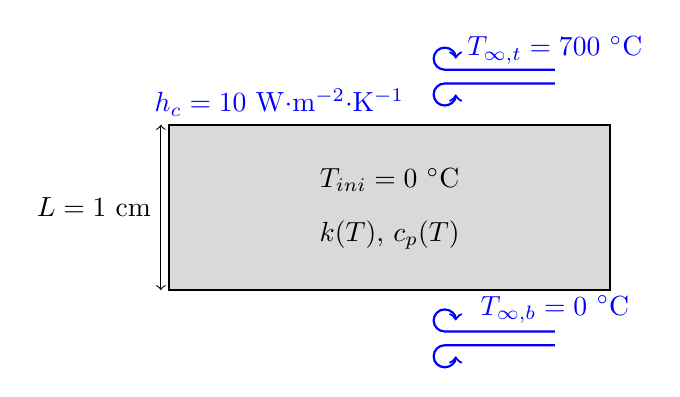
\begin{tikzpicture}[scale=0.7]

\draw[fill=gray!30,thick] (0,0) rectangle (8,3);
\node at (4,2) {$T_{ini} = 0~^\circ\mathrm{C}$};
\node at (4,1) {$k(T)$, $c_p(T)$};

\draw[<->] (-0.15,0) -- (-0.15,3);
\node[left] at (-0.15,1.5) {$L = 1$~cm};

% Convective arrows
\draw[->,thick, blue] (7,3.75) -- (5,3.75) arc[start angle=90, end angle=360, radius=0.2cm];
\draw[->,thick, blue] (7,4) -- (5,4) arc[start angle=270, end angle=0, radius=0.2cm];

\node[blue] at (2,3.4) {$h_c = 10~\mathrm{W{\cdot}m^{-2}{\cdot}K^{-1}}$};
\node[blue] at (7,4.35) {$T_{\infty,t} = 700~^\circ\mathrm{C}$};

\draw[->,thick, blue] (7,-1) -- (5,-1) arc[start angle=90, end angle=360, radius=0.2cm];
\draw[->,thick, blue] (7,-0.75) -- (5,-0.75) arc[start angle=270, end angle=0, radius=0.2cm];

\node[blue] at (7,-0.35) {$T_{\infty,b} = 0~^\circ\mathrm{C}$};

\end{tikzpicture}
\caption{Configuration schematic}
\label{fig:heat_conduction_kc_configuration}
\end{minipage}
\hfill
\begin{minipage}{0.48\textwidth}
\centering
\includegraphics[width=\textwidth]{heat_conduction_kc_results.png}
\caption{Evolution of front and back temperatures with time}
\label{fig:heat_conduction_kc_results}
\end{minipage}

\end{figure}



\ifdefined\standalone
\bibliographystyle{unsrt}
\bibliography{heat_conduction_kc}
\end{document}
\fi


\newpage
\ifdefined\standalone
\documentclass[12pt]{article}
\usepackage{graphicx}
\usepackage{float}
\usepackage[a4paper, margin=1in]{geometry}
\usepackage[utf8]{inputenc}
\usepackage{textcomp}
\usepackage{amsmath}
\usepackage[hidelinks]{hyperref}
\usepackage{tikz}
\usetikzlibrary{decorations.pathmorphing,patterns}
\begin{document}
\fi

\section{Convective Cooling}

This case investigates one-dimensional transient heat conduction in a thick slab of thickness $L = 1~\mathrm{m}$. 
The slab is initially at a uniform temperature of $T_{ini} = 1000~^\circ\mathrm{C}$ and is exposed to ambient air at 
$T_\infty = 0~^\circ\mathrm{C}$ on one face. Heat exchange at the exposed surface occurs by convection and is characterized 
by a heat transfer coefficient $h_c = 1~\mathrm{W\,m^{-2}\,K^{-1}}$. 
The opposite face is assumed to be perfectly insulated. 
The configuration is illustrated in Figure~\ref{fig:heat_conduction_configuration}. 
The thermophysical properties of the slab material are summarized in Table~\ref{tab:thermal_properties_heat_conduction}.

The numerical results are presented in Figure~\ref{fig:heat_conduction_results} and are compared with the analytical solution 
reported by Incropera et al.~\cite{incropera_fundamentals_2007}, which follows the same formulation as 
Equation~\ref{Eq:Thermal_thranscendantale}.

\begin{table}[H]
\centering
\caption{Thermophysical properties of the slab material.}
\label{tab:thermal_properties_heat_conduction}
\renewcommand{\arraystretch}{1.3}
\begin{tabular}{c c c}
\hline
$k$ ($\mathrm{W\,m^{-1}\,K^{-1}}$) &
$c_p$ ($\mathrm{J\,kg^{-1}\,K^{-1}}$) &
$\rho$ ($\mathrm{kg\,m^{-3}}$) \\
\hline
1 & 1 & 1000 \\
\hline
\end{tabular}
\end{table}

\begin{figure}[H]
\centering
\begin{minipage}[t]{0.48\textwidth}
\centering
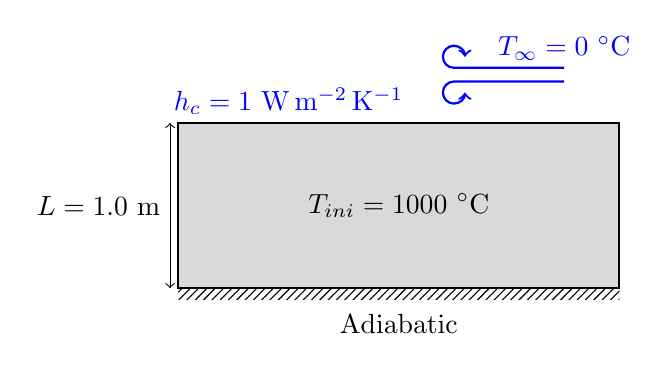
\begin{tikzpicture}[scale=0.7]

\draw[fill=gray!30,thick] (0,0) rectangle (8,3); 
\node at (4,1.5) {$T_{ini} = 1000~^\circ\mathrm{C}$};

\draw[<->] (-0.15,0) -- (-0.15,3);
\node[left] at (-0.15,1.5) {$L=1.0~\mathrm{m}$};

\draw[->,thick, blue] (7,3.75) -- (5,3.75) 
arc[start angle=90, end angle=360, radius=0.2cm]; 
\draw[->,thick, blue] (7,4) -- (5,4) 
arc[start angle=270, end angle=0, radius=0.2cm]; 

\node[blue] at (2,3.4) {$h_c = 1~\mathrm{W\,m^{-2}\,K^{-1}}$};
\node[blue] at (7,4.35) {$T_\infty = 0~^\circ\mathrm{C}$};

\fill[pattern=north east lines] (0,-0.2) rectangle (8,0);
\node[below] at (4,-0.3) {Adiabatic};

\end{tikzpicture}
\caption{Schematic representation of the heat conduction configuration.}
\label{fig:heat_conduction_configuration}
\end{minipage}
\hfill
\begin{minipage}[t]{0.48\textwidth}
\centering
\includegraphics[width=\textwidth]{convective_cooling.png}
\caption{Temporal evolution of temperature at different locations within the solid.}
\label{fig:heat_conduction_results}
\end{minipage}
\end{figure}


\ifdefined\standalone
\end{document}
\fi


\newpage
\ifdefined\standalone
\documentclass[12pt]{article}
\usepackage[a4paper, margin=1in]{geometry}
\usepackage[utf8]{inputenc}
\usepackage{textcomp}
\usepackage{amsmath}
\usepackage{graphicx}
\usepackage{float}
\usepackage[hidelinks]{hyperref}
\usepackage{tikz}
\usetikzlibrary{decorations.pathmorphing,patterns}
\begin{document}
\fi

\section{Insulated Multi-Layer Steel Plate}

This case considers steady-state one-dimensional heat conduction through a multilayer composite slab composed of a central steel layer of thickness $L_{\text{steel}} = 1~\mathrm{cm}$, symmetrically covered by two insulation layers of thickness $L_{\text{ins}} = 2~\mathrm{cm}$ each. The assembly is subjected to asymmetric convective boundary conditions: the hot-side surface is exposed to ambient air at $T_{\infty,t} = 480~^\circ\mathrm{C}$, while the cold-side surface is exposed to air at $T_{\infty,b} = 20~^\circ\mathrm{C}$. The slab is heated for a sufficiently long duration (10~hours) to ensure steady-state conditions. The convective heat transfer coefficient is assumed identical on both sides and equal to $h_c = 10~\mathrm{W\,m^{-2}\,K^{-1}}$ (see Fig.~\ref{fig:isp_fixed_configuration}). The thermophysical properties of the materials are summarized in Table~\ref{tab:thermal_properties_insulated_steel_plate}.

\begin{table}[H]
\centering
\caption{Thermophysical properties of the materials.}
\label{tab:thermal_properties_insulated_steel_plate}
\renewcommand{\arraystretch}{1.3}
\begin{tabular}{l c c c}
\hline
Material &
$k$ ($\mathrm{W\,m^{-1}\,K^{-1}}$) &
$c_p$ ($\mathrm{J\,kg^{-1}\,K^{-1}}$) &
$\rho$ ($\mathrm{kg\,m^{-3}}$) \\
\hline
Steel        & 50.0 & 500  & 7500 \\
Insulation  & 0.2  & 1000 & 200  \\
\hline
\end{tabular}
\end{table}

At steady state, the heat flux is constant through the slab and is given by \cite{incropera_fundamentals_2007}:
\begin{equation}
q'' =
\frac{T_{\infty,t} - T_{\infty,b}}{
\frac{1}{h_c}
+ \frac{L_{\text{ins}}}{k_{\text{ins}}}
+ \frac{L_{\text{steel}}}{k_{\text{steel}}}
+ \frac{L_{\text{ins}}}{k_{\text{ins}}}
+ \frac{1}{h_c}}
\end{equation}

The temperature field within each layer is piecewise linear between successive interfaces, and the temperatures at the interfaces are expressed as: 
\begin{equation}
\left\{
\begin{aligned}
T_0 &= T_{\infty,t} - \frac{q''}{h_c}
&& \text{: hot-side surface temperature}\\
T_1 &= T_0 - q'' \frac{L_{\text{ins}}}{k_{\text{ins}}}
&& \text{: interface between hot-side insulation and steel}\\
T_2 &= T_1 - q'' \frac{L_{\text{steel}}}{k_{\text{steel}}}
&& \text{: interface between steel and cold-side insulation}\\
T_3 &= T_2 - q'' \frac{L_{\text{ins}}}{k_{\text{ins}}}
&& \text{: cold-side surface temperature}
\end{aligned}
\right.
\end{equation}

\begin{figure}[H]
\centering

\begin{minipage}{0.48\textwidth}
    \centering
    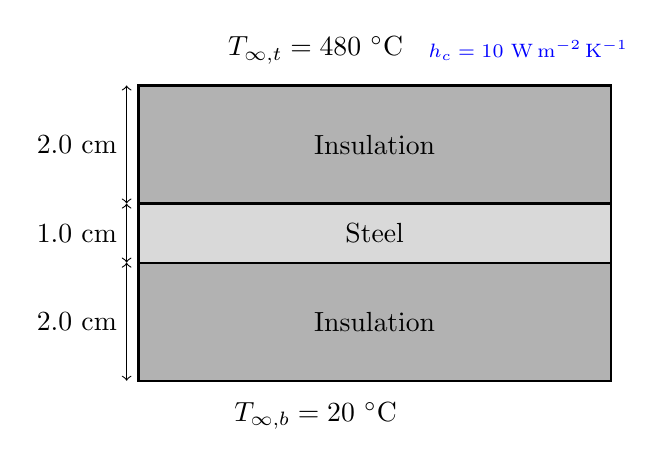
\begin{tikzpicture}[scale=0.75]

    % Steel
    \draw[fill=gray!30,thick] (0,0) rectangle (8,1);
    \node at (4,0.5) {Steel};

    % Bottom insulation (cold side)
    \draw[fill=gray!60,thick] (0,-2) rectangle (8,0);
    \node at (4,-1) {Insulation};
    \node[below] at (3,-2.2) {$T_{\infty,b} = 20~^\circ\mathrm{C}$};

    % Top insulation (hot side)
    \draw[fill=gray!60,thick] (0,1) rectangle (8,3);
    \node at (4,2) {Insulation};
    \node[above] at (3,3.2) {$T_{\infty,t} = 480~^\circ\mathrm{C}$};

    % Dimensions
    \draw[<->] (-0.2,0) -- (-0.2,1);
    \node[left] at (-0.2,0.5) {$1.0~\mathrm{cm}$};

    \draw[<->] (-0.2,-2) -- (-0.2,0);
    \node[left] at (-0.2,-1) {$2.0~\mathrm{cm}$};

    \draw[<->] (-0.2,1) -- (-0.2,3);
    \node[left] at (-0.2,2) {$2.0~\mathrm{cm}$};

    % Convection annotation
    \node[blue] at (6.6,3.6) {\scriptsize $h_c = 10~\mathrm{W\,m^{-2}\,K^{-1}}$};

    \end{tikzpicture}
    \caption{Schematic of the insulated steel plate configuration.}
    \label{fig:isp_fixed_configuration}
\end{minipage}
\hfill
\begin{minipage}{0.48\textwidth}
    \centering
    \includegraphics[width=\textwidth]{insulated_steel_plate.png}
    \caption{Temperature profile as a function of depth within the multilayer slab.}
    \label{fig:temperature_profile}
\end{minipage}

\end{figure}

\ifdefined\standalone
\end{document}
\fi



\newpage
\ifdefined\standalone 
\documentclass[12pt]{article}
\usepackage{graphicx}
\usepackage{float}
\usepackage[a4paper, margin=1in]{geometry}
\usepackage[utf8]{inputenc}
\usepackage{textcomp}
\usepackage{amsmath}
\usepackage{booktabs}
\usepackage{tikz}
\usepackage{enumitem}
\usetikzlibrary{decorations.pathmorphing,patterns}
\usepackage[hidelinks]{hyperref} % <- hypertext

\begin{document}
\fi

\section{Fixed temperatures at boundaries}

A slab of thickness $L = 10~\mathrm{cm}$ is considered. Constant temperatures are imposed at the boundaries, with a temperature of $T_{\infty,t} = 400~^\circ\mathrm{C}$ at the top surface and $T_{\infty,b} = 20~^\circ\mathrm{C}$ at the bottom surface. The initial temperature of the slab is $T_{ini}=0~^\circ\mathrm{C}$, as illustrated in Figure~\ref{fig:ref_fixed_configuration}. The thermophysical properties of the material used in the simulation are reported in Table~\ref{tab:phys_props_fixed}.

The numerical results are validated against the analytical solution given by Incropera et al.~\cite{incropera_fundamentals_2007}. The analytical temperature distribution is expressed as:
\begin{equation}
T(z,t) = T_{\mathrm{ss}}(z) + \sum_{n=1}^{\infty} 
C_n \sin\left( \frac{n \pi z}{L} \right) 
\exp\left[ - \alpha \left( \frac{n \pi}{L} \right)^2 t \right]
\label{eq:T_xt_fixed_bc}
\end{equation}
where the steady-state temperature profile is
\begin{equation}
T_{\mathrm{ss}}(z) = T_{\infty,t} + \frac{T_{\infty,b} - T_{\infty,t}}{L}\, z
\end{equation}
and the Fourier coefficients are given by
\begin{equation}
C_n = \frac{2}{n\pi} 
\left[ 
(T_{ini} - T_{\infty,t}) + (T_{ini} - T_{\infty,b})(-1)^{n+1} 
\right]
\label{eq:Cn}
\end{equation}
Here, $T_0$ denotes the initial uniform temperature of the slab, and $\alpha = k / (\rho c_p)$ is the thermal diffusivity.

 A comparison between numerical and analytical temperature profiles is presented in Figure~\ref{fig:ref_fixed_temp}.

\begin{table}[H]
\centering
\caption{Thermophysical properties of the slab material}
\label{tab:phys_props_fixed}
\renewcommand{\arraystretch}{1.3}
\begin{tabular}{c c c c}
\hline
$k$ ($\mathrm{W\,m^{-1}\,K^{-1}}$) & 
$c_p$ ($\mathrm{J\,kg^{-1}\,K^{-1}}$) & 
$\rho$ ($\mathrm{kg\,m^{-3}}$) & 
$\varepsilon$ ($-$) \\
\hline
0.10 & 1000 & 100 & 0.0 \\
\hline
\end{tabular}
\end{table}

\begin{figure}[H]
\centering
\begin{minipage}[t]{0.45\textwidth}
\centering
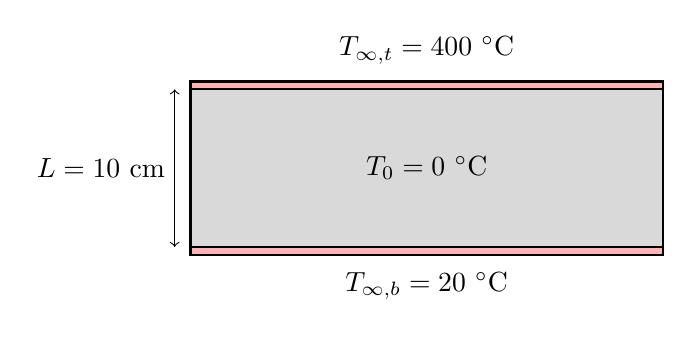
\begin{tikzpicture}[scale=1.0]
\draw[fill=gray!30,thick] (0,0) rectangle (6,2); 
\node at (3,1) {$T_0= 0~^\circ\mathrm{C}$};

\draw[fill=red!30,thick] (0,-0.1) rectangle (6,0);
\node[below] at (3,-0.2) {$T_{\infty,b} = 20~^\circ\mathrm{C}$}; 

\draw[fill=red!30,thick] (0,2) rectangle (6,2.1);
\node[above] at (3,2.2) {$T_{\infty,t} = 400~^\circ\mathrm{C}$};

\draw[<->] (-0.2,0) -- (-0.2,2);
\node[left] at (-0.2,1) {$L=10~\mathrm{cm}$};
\end{tikzpicture}
\caption{Schematic of the slab with fixed temperature boundary conditions}
\label{fig:ref_fixed_configuration}
\end{minipage}
\hfill
\begin{minipage}[t]{0.45\textwidth}
\centering
\includegraphics[width=\linewidth]{fixed_temp.png}
\caption{Comparison between numerical and analytical temperature evolution}
\label{fig:ref_fixed_temp}
\end{minipage}
\end{figure}

\ifdefined\standalone
\bibliographystyle{unsrt}
\bibliography{fixed_temp}
\end{document}
\fi








\newpage
\ifdefined\standalone
\documentclass[12pt]{article}
\usepackage{graphicx}
\usepackage{float}    % <-- For [H] figure placement
\usepackage[a4paper, margin=1in]{geometry} % <-- For better margins
\usepackage[utf8]{inputenc}
\usepackage{textcomp}  % <-- for \textdegree
\usepackage{amsmath}
\usepackage[hidelinks]{hyperref} % <- hypertext
\usepackage{tikz}
\usetikzlibrary{decorations.pathmorphing,patterns}

\begin{document}
\fi

\section{Radiative heat losses}


This verification case investigates a hot plate losing heat solely through thermal re-radiation, which is modeled using the Stefan--Boltzmann law:
\begin{equation}
q''_{\mathrm{r,out}} = \varepsilon \sigma \left( T_s^4 - T_{\infty,t}^4 \right)
\end{equation}
where $T_s$ denotes the surface temperature, $\varepsilon$ is the surface emissivity, and $\sigma$ is the Stefan--Boltzmann constant. The key parameters associated with each subcases are summarized in Table~\ref{tab:phys_props_radloss}.

Two subcases are considered, corresponding to different ambient temperatures: $T_{\infty,t} = 0~^\circ\mathrm{K}$ and $T_{\infty,t} = 273.15~^\circ\mathrm{K}$. In both configurations, the plate is initially at a uniform temperature of $T_0 = 500~^\circ\mathrm{K}$. One surface of the plate is assumed to be adiabatic, while the back surface is exposed to the surroundings. A schematic representation of the computational configuration is provided in Figure~\ref{fig:radloss_configuration}.

The temporal evolution of the temperature profiles is presented in Figure~\ref{fig:rad_loss}. Since no analytical solution is available for this configuration, the numerical results are compared against simulations performed with \textsc{FDS}.

\vspace{-0.5cm}


\begin{table}[H]
\centering
\caption{Thermophysical properties}
\label{tab:phys_props_radloss}
\renewcommand{\arraystretch}{1.3} % spacing between rows
\begin{tabular}{c c c c c c}
\hline
Case &
T$_\infty$ (K) &
$k$ ($\mathrm{W\,m^{-1}\,K^{-1}}$) & 
$c_p$ ($\mathrm{kJ\,kg^{-1}\,K^{-1}}$) & 
$\rho$ ($\mathrm{kg\,m^{-3}}$) & 
$\epsilon (-)$ \\
\hline
1 & 0 & 0.186 & 1.764 & 380 & 1.0 \\
\hline
2 & 273.15 & 0.186 & 1.764 & 380 & 1.0 \\
\hline
\end{tabular}
\end{table}
\vspace{-0.5cm}


\begin{figure}[H]
\centering
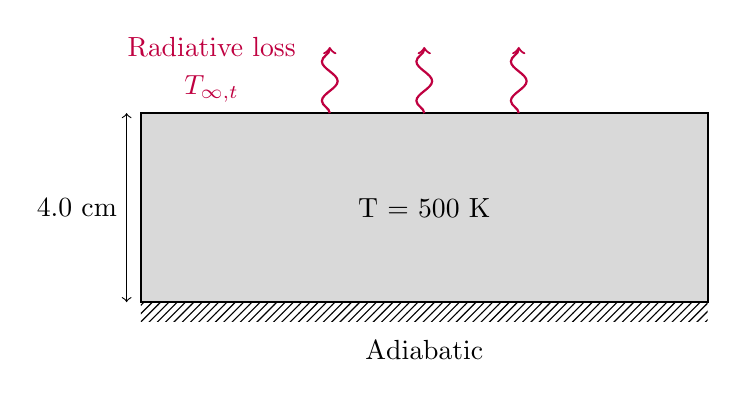
\begin{tikzpicture}[scale=1.2]
\draw[fill=gray!30,thick] (0,0) rectangle (6,2); 
\node at (3,1) {T = 500 K};

\fill[pattern=north east lines] (0,-0.2) rectangle (6,0);
\node[below] at (3,-0.3) {Adiabatic};

\draw[<->] (-0.15,0) -- (-0.15,2);
\node[left] at (-0.15,1) {4.0~cm};

\foreach \x in {1.8,2.8,3.8}
    \draw[purple,thick,->,decorate,decoration={snake,amplitude=1mm,segment length=5mm}] (\x+0.2,2) -- (\x+0.2,2.7);

\node[above,purple] at (0.75,2.5) { Radiative loss};
\node[below,purple] at (0.75,2.5) {$T_{\infty,t}$};
\end{tikzpicture}
\caption{Configuration schematic}
\label{fig:radloss_configuration}
\end{figure}


\begin{figure}[H]
\centering
\includegraphics[width=0.48\textwidth]{radiation_loss_tg0K.png}
\includegraphics[width=0.48\textwidth]{radiation_loss_tg0C.png}
\vspace{-0.5cm}
\caption{Temperature evolution for Case 1 (left) and 2 (right).}
\label{fig:rad_loss}
\end{figure}


\ifdefined\standalone
\end{document}
\fi



\newpage
\ifdefined\standalone 
\documentclass[12pt]{article}
\usepackage{graphicx}
\usepackage{float}
\usepackage[a4paper, margin=1in]{geometry}
\usepackage[utf8]{inputenc}
\usepackage{textcomp}
\usepackage{amsmath}
\usepackage{booktabs}
\usepackage{tikz}
\usepackage{enumitem}
\usetikzlibrary{decorations.pathmorphing,patterns}
\usepackage[hidelinks]{hyperref} % <- hypertext

\begin{document}
\fi

\section{Fixed heat flux boundary condition}
\label{case:rad_1d}


This verification case examines one-dimensional heat conduction in a slab subjected to a prescribed surface heat flux. A slab of thickness $4~\mathrm{cm}$ is initially at a uniform temperature of $T_{ini} = 27~^\circ\mathrm{C}$. The exposed surface is subjected to a constant incident heat flux of $q''_{\mathrm{ext}} = 2~\mathrm{kW\,m^{-2}}$. The material is assumed to be opaque, such that no in-depth radiation penetration occurs. The opposite surface is considered adiabatic, as illustrated in Figure~\ref{fig:rad1d_configuration}. The thermophysical properties of the material are summarized in Table~\ref{tab:phys_props_rad}.

The numerical results are validated against the analytical solution for transient heat conduction in a semi-infinite slab subjected to a constant surface heat flux, as presented by Incropera et al.~\cite{incropera_fundamentals_2007}. The analytical solution is given by:

\begin{equation}
T(z,t) - T_{ini} =
\frac{2 \varepsilon q''_{\mathrm{ext}}}{k}
\left( \frac{\alpha t}{\pi} \right)^{1/2}
\exp\left( -\frac{z^2}{4 \alpha t} \right)
-
\frac{\varepsilon q''_{\mathrm{ext}} z}{k}
\, \mathrm{erfc}\!\left( \frac{z}{2\sqrt{\alpha t}} \right)
\label{eq:T_xt}
\end{equation}
where $\alpha = k / (\rho c_p)$ is the thermal diffusivity, $\varepsilon$ is the surface emissivity, and $x$ denotes the distance from the exposed surface.


\begin{table}[H]
\centering
\caption{Thermophysical properties used in the simulation}
\label{tab:phys_props_rad}
\renewcommand{\arraystretch}{1.3}
\begin{tabular}{c c c c}
\hline
$k$ ($\mathrm{W\,m^{-1}\,K^{-1}}$) &
$c_p$ ($\mathrm{kJ\,kg^{-1}\,K^{-1}}$) &
$\rho$ ($\mathrm{kg\,m^{-3}}$) &
$\varepsilon$ ($-$) \\
\hline
0.186 & 1.764 & 380 & 1.0 \\
\hline
\end{tabular}
\end{table}

\begin{figure}[H]
\centering
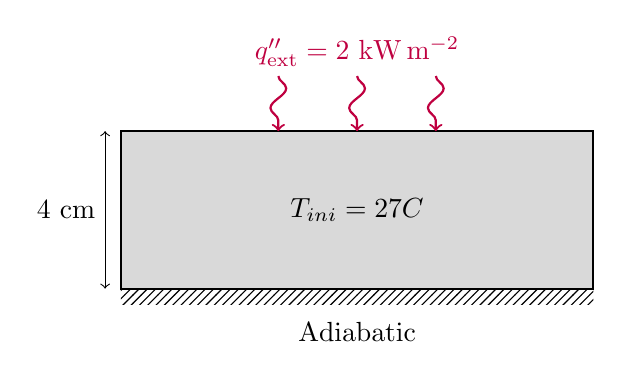
\begin{tikzpicture}[scale=1]
\draw[fill=gray!30,thick] (0,0) rectangle (6,2);
\node at (3,1) {$T_{ini}=27°C$};

\fill[pattern=north east lines] (0,-0.2) rectangle (6,0);
\node[below] at (3,-0.3) {Adiabatic};

\draw[<->] (-0.2,0) -- (-0.2,2);
\node[left] at (-0.2,1) {$4~\mathrm{cm}$};

\foreach \x in {1.8,2.8,3.8}
  \draw[purple,thick,->,decorate,decoration={snake,amplitude=1mm,segment length=5mm}]
  (\x+0.2,2.7) -- (\x+0.2,2);

\node[above,purple] at (3,2.7) { $q''_{\mathrm{ext}} = 2~\mathrm{kW\,m^{-2}}$};
\end{tikzpicture}
\caption{Schematic representation of the computational configuration.}
\label{fig:rad1d_configuration}
\end{figure}





\begin{figure}[H]
\centering
\includegraphics[width=0.6\textwidth]{radiation_1d.png}
\vspace{-0.4cm}
\caption{Temperature evolution at different depths inside the slab.}
\label{fig:rad_1d}
\end{figure}




\ifdefined\standalone
\bibliographystyle{unsrt}
\bibliography{radiation_1d}
\end{document}
\fi








\newpage
\ifdefined\standalone 
\documentclass[12pt]{article}
\usepackage{graphicx}
\usepackage{float}
\usepackage[a4paper, margin=1in]{geometry}
\usepackage[utf8]{inputenc}
\usepackage{textcomp}
\usepackage{amsmath}
\usepackage{booktabs}
\usepackage{tikz}
\usepackage{enumitem}
\usetikzlibrary{decorations.pathmorphing,patterns}
\usepackage[hidelinks]{hyperref} % <- hypertext
\usepackage{caption}

\begin{document}
\fi

\section{In-depth radiation absorption}

This verification case is designed to assess the capability of \textt{Gpyro} to accurately model one-dimensional radiative heat absorption in a semi-opaque material. A slab of thickness $10~\mathrm{cm}$ is subjected exclusively to an incident radiative heat flux of $q''_{\mathrm{ext}} = 5~\mathrm{kW\,m^{-2}}$, which penetrates the material. The slab is assumed to be semi-opaque and characterized by a constant absorption coefficient $\kappa = 24~\mathrm{m^{-1}}$. Under these assumptions, the volumetric radiative heat source resulting from in-depth radiation absorption is described by an Beer-Lambert law:
\begin{equation}
\dot{Q}''_r(z) = \varepsilon \kappa q''_{\mathrm{ext}} \exp\left( -\kappa z \right)
\end{equation}
where $z$ denotes the distance from the irradiated surface and $\varepsilon$ is the surface emissivity.
Three configurations are considered: radiation applied at the top surface, at the bottom surface, and at both surfaces simultaneously. For each case, numerical results (annotated Gpyro latest) are compared with the corresponding analytical solution and with results obtained using the original version of \texttt{Gpyro} (annotated Gpyro V0.8). The thermophysical properties and simulation parameters are listed in Table~\ref{tab:simu_props_raddepth}.


\begin{table}[H]
\centering
\small
\caption{Simulation properties}
\label{tab:simu_props_raddepth}
\renewcommand{\arraystretch}{1.3}
\begin{tabular}{c c c c c c}
\hline
$k$ ($\mathrm{W\,m^{-1}\,K^{-1}}$) & 
$c_p$ ($\mathrm{J\,kg^{-1}\,K^{-1}}$) & 
$\rho$ ($\mathrm{kg\,m^{-3}}$) & 
$\varepsilon$ ($-$) &
$\kappa$ ($\mathrm{m^{-1}}$) &
$q''_{\mathrm{ext}}$ ($\mathrm{kW\,m^{-2}}$) \\
\hline
0.10 & 1000 & 100 & 1.0 & 24 & 5 \\
\hline
\end{tabular}
\end{table}


\begin{figure}[H]
\centering

% ---- First row ----
\begin{minipage}[t]{0.48\textwidth}
\centering
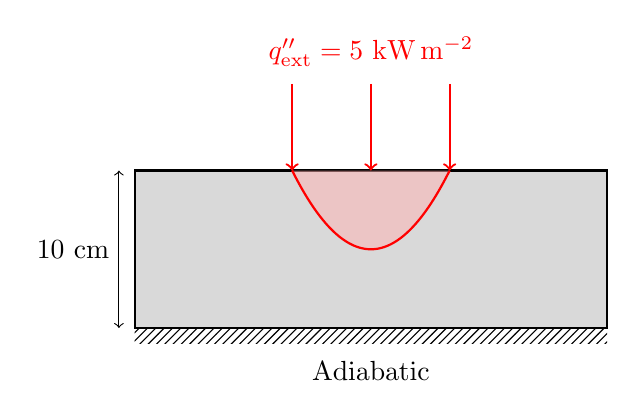
\begin{tikzpicture}[scale=1.0]
% Slab
\draw[fill=gray!30,thick] (0,0) rectangle (6,2);

% Adiabatic bottom
\fill[pattern=north east lines] (0,-0.2) rectangle (6,0);
\node[below] at (3,-0.3) {Adiabatic};

% Thickness
\draw[<->] (-0.2,0) -- (-0.2,2);
\node[left] at (-0.2,1) {10~cm};

% Incident radiation
\foreach \x in {1.8,2.8,3.8}
  \draw[->,thick,red] (\x+0.2,3.1) -- (\x+0.2,2);

\node[above,red] at (3,3.2) {$q''_{\mathrm{ext}} = 5~\mathrm{kW\,m^{-2}}$};

% Absorption profile
\fill[red!30, opacity=0.5, domain=2:4, variable=\x]
  (2,2) plot ({\x}, {(\x-3)^2 + 1}) -- (4,2) -- cycle;

\draw[thick, red, domain=2:4, samples=100]
  plot ({\x}, {(\x-3)^2 + 1});
\end{tikzpicture}
\caption*{(a) Configuration schematic}
\end{minipage}
\hfill
\begin{minipage}[t]{0.48\textwidth}
\centering
\includegraphics[width=\linewidth]{top_flux_results.png}
\caption*{(b) Top irradiation}
\end{minipage}

\begin{minipage}[t]{0.48\textwidth}
\centering
\includegraphics[width=\linewidth]{bottom_flux_results.png}
\caption*{(c) Bottom irradiation}
\end{minipage}
\hfill
\begin{minipage}[t]{0.48\textwidth}
\centering
\includegraphics[width=\linewidth]{double_flux_results.png}
\caption*{(d) Double-sided irradiation}
\end{minipage}

\caption{Comparison between Gpyro and analytical solutions for in-depth radiation.}
\label{fig:flow_comparison}
\end{figure}



\ifdefined\standalone
\end{document}
\fi








\newpage
\ifdefined\standalone 
\documentclass[12pt]{article}
\usepackage{graphicx}
\usepackage{float}
\usepackage[a4paper, margin=1in]{geometry}
\usepackage[utf8]{inputenc}
\usepackage{textcomp}
\usepackage{amsmath}
\usepackage{booktabs}
\usepackage{tikz}
\usepackage{enumitem}
\usetikzlibrary{decorations.pathmorphing,patterns}
\usepackage[hidelinks]{hyperref} % <- hypertext
\usepackage{caption}

\begin{document}
\fi

\section{In-Depth Radiation With Surface Convection}

This verification case assesses the ability of Gpyro to represent one-dimensional heat absorption due to volumetric radiation combined with surface cooling by convection. A slab of thickness $L = 10~\mathrm{cm}$ is considered.The thermophysical properties of the material are summarized in Table~\ref{tab:rad_conv_phys_props}. The top surface is subjected to convective heat transfer with a constant convective heat transfer coefficient of $h_c = 10~\mathrm{W\,m^{-2}\,K^{-1}}$ and an ambient gas temperature of $T_\infty = 25~^\circ\mathrm{C}$. In addition, the top surface is also exposed to an external radiative heat flux of $q''_\mathrm{ext} = 5~\mathrm{kW\,m^{-2}}$.The material is assumed to be semi-transparent, characterized by an absorption coefficient of $\kappa = 24~\mathrm{m^{-1}}$. The bottom surface of the slab is assumed to be adiabatic. The initial temperature is uniform throughout the material, with $T_{ini} = 25~^\circ\mathrm{C}$. The configuration is illustrated in Fig.~\ref{fig:rad_conv_temp}.

An analytical solution for transient temperature evolution within the slab is available and is taken from the formulation presented in Lautenberger’s thesis \cite{lautenberger2007}:

\begin{equation}
\label{eq:temp_depth_lautenberger}
\begin{aligned}
T(z) - T_{ini} &= \frac{2 \varepsilon q''_\mathrm{ext} \kappa^2}{k}
\sum_{m=1}^{\infty} \frac{1}{\lambda_m (\kappa^2 + \lambda_m^2)} \\
&\quad \times
\frac{\cos(\lambda_m L) + \tfrac{\lambda_m}{\kappa} \sin(\lambda_m L) - \exp(-\kappa L)}
{\lambda_m L + \tfrac{1}{2} \sin(2 \lambda_m L)} \\
&\quad \times
\cos\!\bigl(\lambda_m (L - z)\bigr)
\left(1 - \exp(-\alpha \lambda_m^2 t)\right)
\end{aligned}
\end{equation}

The eigenvalues $\lambda_m$ are obtained by solving the following equation:

\begin{equation}
\label{eq:lambda_condition}
\cot(\lambda_m L) = \frac{k}{h_c}\,\lambda_m
\end{equation}


\begin{table}[H]
\centering
\caption{Material properties}
\label{tab:rad_conv_phys_props}
\renewcommand{\arraystretch}{1.2}
\begin{tabular}{c c c c c}
\hline
$k$ ($\mathrm{W\,m^{-1}\,K^{-1}}$) &
$c_p$ ($\mathrm{J\,kg^{-1}\,K^{-1}}$) &
$\rho$ ($\mathrm{kg\,m^{-3}}$) &
$\varepsilon$ &
$\kappa$ (m$^{-1}$) \\
\hline
0.10 & 1000 & 100 & 1 & 24 \\
\hline
\end{tabular}
\end{table}


\begin{figure}[H]
\centering

\begin{minipage}[t]{0.45\textwidth}
\centering
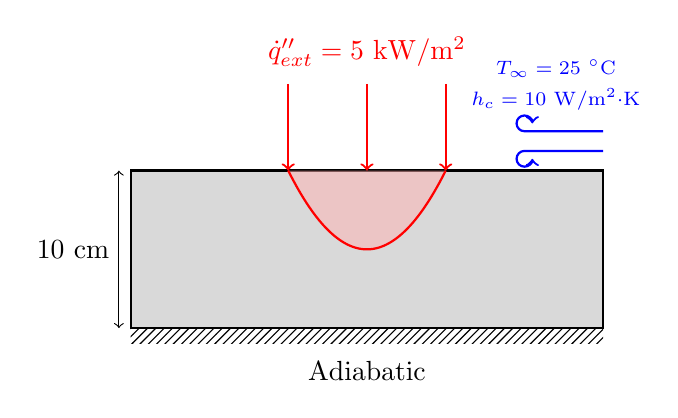
\begin{tikzpicture}[scale=1.0]
% MDF block
\draw[fill=gray!30,thick] (0,0) rectangle (6,2); 

% Adiabatic bottom
\fill[pattern=north east lines] (0,-0.2) rectangle (6,0);
\node[below] at (3,-0.3) {Adiabatic};

% Dimension line for height
\draw[<->] (-0.15,0) -- (-0.15,2);
\node[left] at (-0.15,1) {10~cm};

\foreach \x in {1.8,2.8,3.8}
    \draw[->,thick,red] (\x+0.2,3.1) -- (\x+0.2,2);

\node[above,red] at (3,3.2) {$\dot{q}''_{ext} = 5~\mathrm{kW/m^2}$};

\draw[->,thick, blue] (6,2.25) -- (5,2.25) arc[start angle=90, end angle=360, radius=0.1cm]; 
\draw[->,thick, blue] (6,2.5) -- (5,2.5) arc[start angle=270, end angle=0, radius=0.1cm];

\node[blue] at (5.4,2.9) {\scriptsize $h_c = 10~\mathrm{W/m^2{\cdot}K}$};
\node[blue] at (5.4,3.3) {\scriptsize $T_\infty = 25~^\circ\mathrm{C}$};

\fill[red!30, opacity=0.5, domain=2:4, variable=\x] (2,2) plot ({\x}, {(\x-3)^2 + 1}) --(4,2) -- cycle;

\draw[thick, red, domain=2:4, samples=100, smooth, variable=\x] plot ({\x}, {(\x-3)^2 + 1});

\end{tikzpicture}
\caption{Configuration schematic}
\label{fig:rad_conv_configuration}
\end{minipage}
\hfill
\begin{minipage}[t]{0.45\textwidth}
\centering
    \includegraphics[width=\linewidth]{temperature_results.png}
    \caption{Temperature evolution at different points in the slab}
\label{fig:rad_conv_temp}
\end{minipage}
\end{figure}

\ifdefined\standalone
\end{document}
\fi








\newpage
\ifdefined\standalone 
\documentclass[12pt]{article}
\usepackage{graphicx}
\usepackage{float}
\usepackage[a4paper, margin=1in]{geometry}
\usepackage[utf8]{inputenc}
\usepackage{textcomp}
\usepackage{amsmath}
\usepackage{booktabs}
\usepackage{tikz}
\usepackage{enumitem}
\usetikzlibrary{decorations.pathmorphing,patterns}
\usepackage[hidelinks]{hyperref} % <- hypertext

\begin{document}
\fi

\section{Mixed heat transfer}
This verification case assesses the capability of Gpyro to accurately represent 1D heat transfer involving multiple modes of transfer, and compares the results with those from FDS. The scenario consists of a medium-density fibreboard (MDF) sample subjected to a cone calorimeter test in a nitrogen atmosphere. The properties of the simulated materials can be found in table \ref{tab:phys_props_mdf}. The material is exposed to an external heat flux of $q''_{ext}=1~\mathrm{kW/m^2}$ and ambient air at 25~$^\circ$C, with a convection coefficient of $h_c = 10~\mathrm{W\,m^{-2}\,K^{-1}}$.

\begin{table}[H]
\centering
\caption{Thermophysical properties of MDF}
\label{tab:phys_props_mdf}
\renewcommand{\arraystretch}{1.3} % spacing between rows
\begin{tabular}{c c c c}
\hline
$k$ ($\mathrm{W\,m^{-1}\,K^{-1}}$) & 
$c_p$ ($\mathrm{J\,kg^{-1}\,K^{-1}}$) & 
$\rho$ ($\mathrm{kg\,m^{-3}}$) & 
$\varepsilon (-)$ \\
\hline
0.15 & 1340 & 605 & 0.86 \\
\hline
\end{tabular}
\end{table}

The results obtained using Gpyro are compared to those from FDS. Figure~\ref{fig:mixed_temp} presents the comparison of the temperature evolution in time at various depths.
\begin{figure}[H]
\centering

\begin{minipage}[t]{0.45\textwidth}
\centering
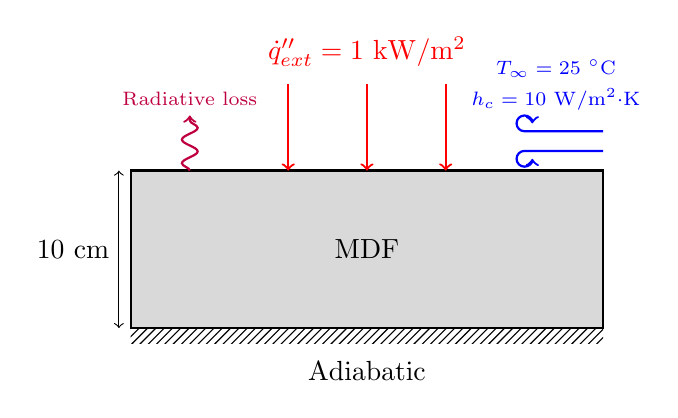
\begin{tikzpicture}[scale=1.0]
% MDF block
\draw[fill=gray!30,thick] (0,0) rectangle (6,2); 
\node at (3,1) {MDF};

% Adiabatic bottom
\fill[pattern=north east lines] (0,-0.2) rectangle (6,0);
\node[below] at (3,-0.3) {Adiabatic};

% Dimension line for height
\draw[<->] (-0.15,0) -- (-0.15,2);
\node[left] at (-0.15,1) {10~cm};

\foreach \x in {1.8,2.8,3.8}
    \draw[->,thick,red] (\x+0.2,3.1) -- (\x+0.2,2);

\node[above,red] at (3,3.2) {$\dot{q}''_{ext} = 1~\mathrm{kW/m^2}$};

\draw[->,thick, blue] (6,2.25) -- (5,2.25) arc[start angle=90, end angle=360, radius=0.1cm]; 
\draw[->,thick, blue] (6,2.5) -- (5,2.5) arc[start angle=270, end angle=0, radius=0.1cm]; 

\node[blue] at (5.4,2.9) {\scriptsize $h_c = 10~\mathrm{W/m^2{\cdot}K}$};
\node[blue] at (5.4,3.3) {\scriptsize $T_\infty = 25~^\circ\mathrm{C}$};

\draw[purple,thick,->,decorate,decoration={snake,amplitude=1mm,segment length=3mm}] (0.75,2) -- (0.75,2.7);

\node[above,purple] at (0.75,2.7) {\scriptsize Radiative loss};
\end{tikzpicture}
\caption{Configuration schematic}
\label{fig:mixed_configuration}
\end{minipage}
\hfill
\begin{minipage}[t]{0.45\textwidth}
\centering
\includegraphics[width=\linewidth]{conv_rad.png}
\caption{Temperature evolution comparison}
\label{fig:mixed_temp}
\end{minipage}
\end{figure}

\ifdefined\standalone
\end{document}
\fi








\ifdefined\ThermalOneD
\end{document}
\fi

